\documentclass[11pt, oneside]{article}   	% use "amsart" instead of "article" for AMSLaTeX format
\usepackage{geometry}                		% See geometry.pdf to learn the layout options. There are lots.
\geometry{letterpaper}                   		% ... or a4paper or a5paper or ... 
%\geometry{landscape}                		% Activate for for rotated page geometry
%\usepackage[parfill]{parskip}    		% Activate to begin paragraphs with an empty line rather than an indent
\usepackage{graphicx}				% Use pdf, png, jpg, or eps� with pdflatex; use eps in DVI mode
								% TeX will automatically convert eps --> pdf in pdflatex		
\usepackage{amssymb}
\usepackage{amsmath}

\title{Spherical Cap - part II}
%\author{The Author}
\date{}							% Activate to display a given date or no date

\graphicspath{{/Users/telliott_admin/Dropbox/Tex/png/}}

\usepackage{listings,relsize} 
\lstloadlanguages{R} 
\lstset{language=R,basicstyle=\smaller[1],commentstyle=\rmfamily\smaller, 
  showstringspaces=false,% 
  xleftmargin=4ex,literate={<-}{{$\leftarrow$}}1 {~}{{$\sim$}}1} 
\lstset{escapeinside={(*}{*)}}   % for (*\ref{ }*) inside lstlistings (S code) 
\begin{document}

\maketitle
%\section{}
% \subsection*{R code}
% \begin{lstlisting}  \end{lstlisting}
% \begin{center} 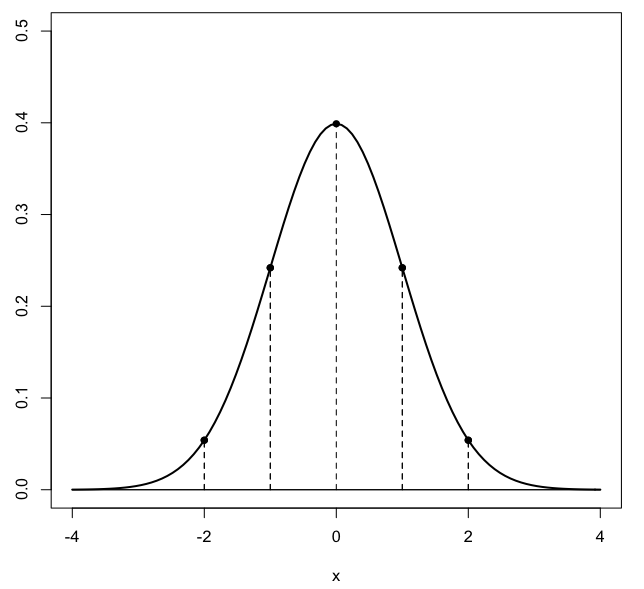
\includegraphics [scale=0.4] {gauss3.png} \end{center}
% \begin{bmatrix} a  &  b \\ c  &  d \end{bmatrix}
% \bigg |_

\large
\noindent
In this write-up I want to show a different derivation of the formula for the volume of a spherical cap.  This is the solid obtained by slicing off a part of a sphere with a plane. 
\begin{center} 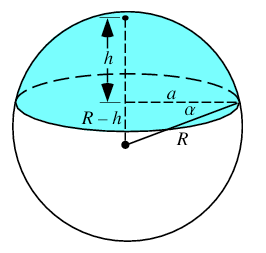
\includegraphics [scale=0.6] {spherical_cap.png} \end{center}
The formula is 
\begin{equation}
\boxed{V_{cap} = \frac{1}{3} \pi h^2(3R - h)}
\end{equation}
\vspace{5 mm}

\noindent
Actually, I will show two different derivations.  The first is perhaps easiest but requires us to know the surface area of the spherical cap.  So that's where we start.

\subsection*{Surface area of the cap}

The formula for the surface area of a part of the sphere is not very complicated.  Amazingly, it doesn't matter whether we are dealing with a spherical cap of height $h$ or a belt around the sphere at the equator with width $h$ (or somewhere in between).  At each point, the surface area is $A = 2\pi Rh$.  Here is a  simple argument.
\vspace{5 mm}

\noindent
If we start from the equator, and think about a thin belt going around the circumference, the belt has length equal to the circumference $2\pi R$ and width $h$, and thus area
\[ A = 2 \pi R h \]
We believe this should be the formula for the surface area of a belt of width $h$, at least near the equator.  In the figure, we have labeled this width as $R-h$, because we are really interested in the cap.  Thus, for the calculation below, this area will be $2\pi R(R-h)$.

Consider that the total surface area of the hemisphere is $2\pi R^2$ so the area of the cap is the difference
\[ A = 2\pi R^2 -  2 \pi R (R-h) = 2 \pi Rh \]
That is, the area of the cap depends only on $R$ and its width (here called $h$).

Furthermore, if we look in the figure at the right triangle with $h$ and $a$ as the sides, then $r$ (not labeled in the figure) is the hypotenuse of that triangle.  It is sometimes called the slant height.  We calculate
\[ a^2 = R^2 - (R - h)^2 = 2 Rh - h^2 \]
\[ r^2 = a^2 + h^2 = 2 Rh - h^2 + h^2 = 2 Rh \]
Now think about a very small spherical cap, then it would be almost flat, a circle, and its radius would be $r$ and area
\[ A = \pi r^2 \]
But $r^2 = 2Rh$, so again we have the same formula for the surface area of a small cap and a belt near the equator!

Now consider a belt of width $h$ at some position which is not close to either the top or the horizontal diameter of this cross-section of the sphere.  In using the formula $A = 2 \pi R h$, if $h$ is the width of the belt on the surface, that suggests that the circumference at this position is $2 \pi R$, which is obviously wrong.  It should be $2\pi a$.

Here's a sketch:
\begin{center} 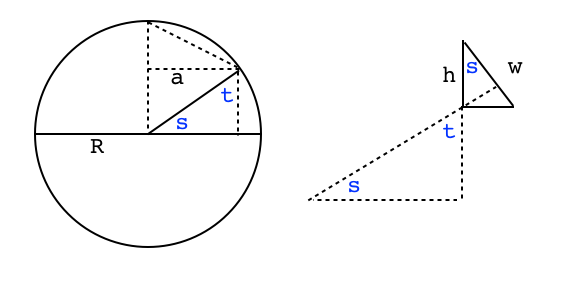
\includegraphics [scale=0.6] {sphcap2.png} \end{center}
We want the area of the spherical belt of height $h$  whose radius is $a$.  The angles are labeled in blue as $s$ and $t$, and they are complementary angles.
\[ a = R \cos s \]
So $a$ is smaller than R by the factor $\cos s$.  In the right panel, we show a small triangle at the surface of the sphere.  The width $w$ is flat on the surface, and since the dotted line is the radius $R$, $R$ makes a right angle where it intercepts $w$.  By complementary angles, we can see that the angle at the top of this triangle is also equal to $s$, so we have the relationship
\[ h = w \cos s \]
So the true area is
\[ 2 \pi a w = 2 \pi R \cos s \frac{h}{\cos s} = 2 \pi R h \]
The cosine of the angle comes in twice, and these factors cancel.  The formula $2\pi R h$ is correct everywhere.

\subsection*{approach through calculus}

As an alternative, I have a derivation from calculus.

The surface area of a volume of revolution is
\[ A = 2 \pi \int y \sqrt{1 + (\frac{dy}{dx})^2} \ dx \]
The square root comes from the surface area element.  This formula looks unwieldy (and often is difficult to work with).  But in this particular case it simplifies dramatically.

If we take a circle as the curve, with formula
\[ x^2 + y^2 = R^2 \]
\[ 2x \ dx + 2y \ dy = 0 \]
\[ \frac{dy}{dx} = - \frac{x}{y} \]
So
\[ A = 2 \pi \int y \ \sqrt{1 + \frac{x^2}{y^2}} \ dx \]
\[ A = 2 \pi \int \sqrt{y^2 + x^2} \ dx \]
\[ A = 2 \pi \int R \ dx = 2 \pi R x \]
Evaluated between $x=a \to x=b$
\[ A = 2 \pi R (b-a) = 2 \pi R h \]

This makes it very clear that the area does not depend where we are on the sphere.  A spherical cap with height $h$ has the same area as a belt of width $h$ wrapped around the equator, or any belt of width $h$ in between the two.

And as we noticed before, the area of a belt or sperical cap, $2 \pi R h$, is equal to the surface area of a cylinder of radius $R$ and height $h$, the so-called hat-box theorem.

\subsection*{Volume of the spherical cap:  method 1}

Once we have the area of the spherical cap, we can calculate the volume fairly easily.  We consider first a spherical segment (the segment of the whole sphere whose surface is the spherical cap).  The volume of the segment is just the volume of the sphere times the fractional area
\[ V_{segment} = \frac{4}{3}\pi R^3 \ \ \frac{2 \pi R h}{4 \pi R^2} = \frac{2}{3} \pi R^2 h \]

The volume of the spherical cap is this volume, minus the volume of the cone with height $R-h$ and base of $\sqrt{R^2 - (R-h)^2}$.  The cone has volume
\[ V_{cone} = \frac{1}{3}\pi (R-h)(R^2-(R-h)^2) \]
Working with the inside part
\[ (R-h)(R^2-(R-h)^2) \]
\[ (R-h)(2Rh - h^2)  \]
\[ 2R^2h - Rh^2 - 2Rh^2 + h^3  \]
\[ 2R^2h - 3Rh^2 + h^3  \]
So
\[ V_{cone} = \frac{1}{3}\pi (2R^2h - 3Rh^2 + h^3) \]
And
\[ V_{cap} = V_{segment} - V_{cone} \]
\[ = \frac{2}{3} \pi R^2 h - \frac{1}{3}\pi (2R^2h - 3Rh^2 + h^3) \]
\[ = \frac{1}{3} \pi (3Rh^2 - h^3) \]
\[ V_{cap} = \frac{1}{3} \pi h^2(3R - h) \]

\subsection*{Volume of the spherical cap:  method 2}

I want to use Archimedes' method to repeat this derivation, so let's review how to do the volume for a normal sphere.  If you remember, it is easy to show that the area of each horizontal slice through the sphere added to that for the inverted cone (at the same height $h$) is equal to the area of a slice of the cylinder (which is a constant).
\begin{center} 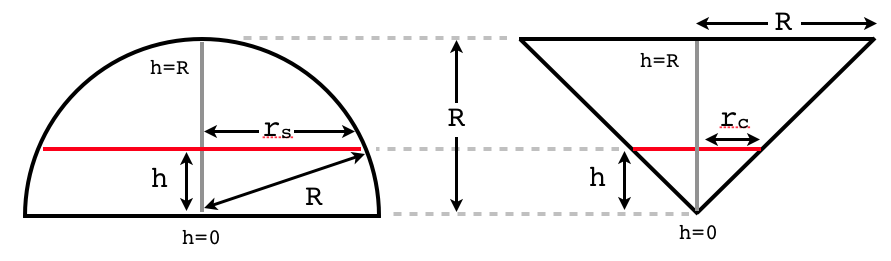
\includegraphics [scale=0.5] {sphere_cone.png} \end{center}

\[ r_{s}^2 = R^2 - h^2 \]
\[ r_{c}^2 = h^2 \]
\[ r_{s}^2 + r_{c}^2 = R^2 \]
Therefore
\[ A_{s} + A_{c} = A_{cyl} \]
To get the volume of a spherical cap, we need to find the volume of the base of the cone after cutting off the top (to form what's called a frustrum).  That volume is the difference between the whole volume of the cone and the volume of the missing top piece.

I didn't redraw the figure above, but to match wikipedia and Wolfram $h$ will need to be the height of the frustrum and $R-h$ the height of the small cone.

\begin{center} 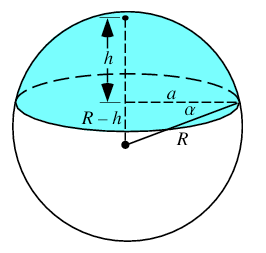
\includegraphics [scale=0.6] {spherical_cap.png} \end{center}

That is, I will use $h$ for the distance from the top of the sphere to the plane which cuts through to form the spherical cap.  The radius of the sphere (and the cone) will be $R$ as before, and the radius at the height $h$ will be $a$. 

From the Pythagorean Theorem, 
\[ a^2 + (R-h)^2 = R^2 \]
\[ a^2 + R^2 - 2hR + h^2 = R^2 \]
\[ R = \frac{a^2 + h^2}{2h} \]
We will use this relationship later in simplifying our formula.

Now the volume of the whole cone is
\[ V_C = \frac{1}{3} \pi R^3 \]
And the volume of the small cone with height $R-h$ is
\[ V_c = \frac{1}{3} \pi (R-h)^3 = \frac{1}{3} \pi (R^3 - 3R^2h + 3Rh^2 - h^3) \]
The difference is the volume of the frustrum
\[ V_{frust} = V_C - V_c = \frac{1}{3} \pi \ [ \ R^3 - R^3 + 3R^2h - 3Rh^2 + h^3 \ ] \ \]
\[ = \frac{\pi}{3} \ [ \ 3R^2h - 3Rh^2 + h^3 \ ] \ \]
The volume of the cylinder is 
\[ V_{cyl} = \pi R^2 h \]
Subtracting the volume of the frustrum, we obtain the volume of the spherical cap
\[ V_{cap} = V_{cyl} - V_{frust} \]
\[ = \pi R^2 h - \frac{1}{3} \pi (3R^2h - 3Rh^2 + h^3) \]
\[ = \frac{\pi}{3} (3Rh^2 - h^3) \]
\begin{equation}
\boxed{V_{cap} = \frac{\pi}{3} h^2 (3R - h)}
\end{equation}
which matches what we had at the top.
\begin{center} 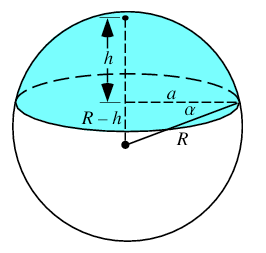
\includegraphics [scale=0.6] {spherical_cap.png} \end{center}
We can get a different form if we substitute for $R$ from above
\[ V_{cap} = \frac{\pi}{3} h^2 \ [ \ 3 \ \frac{a^2 + h^2}{2h} - h\ ] \ \]
\[ V_{cap} = \pi ( \frac{1}{2}a^2h + \frac{1}{2}h^3 - \frac{1}{3}h^3 ] \ \]
\[ V_{cap} = \pi ( \frac{1}{2}a^2h + \frac{1}{6}h^3 ] \ \]
\begin{equation}
\boxed{V_{cap} = \frac{\pi}{6} h (3a^2 + h^2)}
\end{equation}

\end{document}  